\documentclass[letter]{article} 
\addtolength{\hoffset}{-2.25cm}
\addtolength{\textwidth}{4.5cm}
\addtolength{\voffset}{-3.25cm}
\addtolength{\textheight}{5cm}
\setlength{\parskip}{0pt}
\setlength{\parindent}{0in}

\usepackage[square,sort,comma,numbers]{natbib}
\usepackage{blindtext} % Package to generate dummy text
\usepackage{charter} % Use the Charter font
\usepackage[utf8]{inputenc} % Use UTF-8 encoding
\usepackage{microtype} % Slightly tweak font spacing for aesthetics
\usepackage{amsthm, amsmath, amssymb} % Mathematical typesetting
\usepackage{float} % Improved interface for floating objects
\usepackage{hyperref} % For hyperlinks in the PDF
\usepackage{graphicx, multicol} % Enhanced support for graphics
\usepackage{xcolor} % Driver-independent color extensions
\usepackage{pseudocode} % Environment for specifying algorithms in a natural way
\usepackage[ddmmyyyy]{datetime} % Uses YEAR-MONTH-DAY format for dates
\usepackage[spanish, activeacute, es-lcroman]{babel}

\usepackage{fancyhdr} % Headers and footers
\pagestyle{fancy} % All pages have headers and footers
\fancyhead{}\renewcommand{\headrulewidth}{0pt} % Blank out the default header
\fancyfoot[L]{} % Custom footer text
\fancyfoot[C]{} % Custom footer text
\fancyfoot[R]{\thepage} % Custom footer text
\newcommand{\note}[1]{\marginpar{\scriptsize \textcolor{red}{#1}}} % Enables comments in red on margin

\makeatletter
\renewcommand\subsection{\@startsection{subsection}{3}{\z@}%
                                     {-3.25ex\@plus -1ex \@minus -.2ex}%
                                     {-1.5ex \@plus -.2ex}% Formerly 1.5ex \@plus .2ex
                                     {\normalfont\normalsize\bfseries}}
\makeatother

\usepackage{listings}
\lstloadlanguages{[5.2]Mathematica}

\usepackage{enumerate}

\usepackage{subcaption}

\usepackage{dsfont}

\usepackage{wrapfig}

\usepackage{enumitem}

\usepackage{cancel}

\usepackage{booktabs}

\usepackage{caption}
\usepackage{subcaption}

%----------------------------------------------------------------------------------------


%-------------------------------
%	TITLE VARIABLES (identify your work!)
%-------------------------------

\newcommand{\firstname}{Nicolas Maldonado Baracaldo}
\newcommand{\firstid}{201423809}
\newcommand{\firstemail}{n.maldonado10@uniandes.edu.co}

\begin{document}

%-------------------------------
%	TITLE SECTION (do not modify unless you really need to)
%-------------------------------
\fancyhead[C]{}
\hrule \medskip
\begin{minipage}{0.295\textwidth} 
\raggedright
\footnotesize
\firstname \hfill\\ 
\firstid \hfill\\ 
\firstemail \hfill\\
\end{minipage}
\begin{minipage}{0.4\textwidth} 
\centering 
\large 
Estadística No Paramétrica y Remuestreo (MATE3526)\\
\normalsize
Adolfo J. Quiroz\\
Proyecto 2\\
\end{minipage}
\begin{minipage}{0.295\textwidth} 
\raggedleft
\today\hfill\\
\end{minipage}
\medskip\hrule 
\bigskip

\setlength{\parskip}{8pt}
\setlength{\parindent}{0.5in}

%-------------------------------
%	ASSIGNMENT CONTENT (add your responses)
%-------------------------------

En estadística no paramétrica se considera una clase de tests de significancia llamados \emph{tests de permutación}, los cuales consisten en obtener una distribución para un estadístico de prueba bajo la hipótesis nula calculando dicho estadístico para distintas permutaciones de la muestra. En particular pueden permutarse los signos o ángulos de los datos de la muestra como se verá a continuación.

Por otra parte tenemos la noción de simetría multivariada, de las cuales hay varios tipos \cite{SerflingMultivariateAsymmetry}, siendo de particular importancia la simetría de signos y la simetría esférica.

Se dice que $X \in \mathbb{R}^d$ tiene \emph{simetría de signos} cuando $X \overset{(d)}{=} -X$. Se dice que $X \in \mathbb{R}^d$ tiene \emph{simetría
esférica} cuando, para toda matriz ortogonal $d \times d$ $V$, $X \overset{(d)}{=} VX$. La simetría esférica implica simetría de signos pues el requerimiento de la simetría de signos de hecho corresponde a usar algunas matrices ortogonales específicas.

La simetría de signos puede también pensarse en términos de que para todo $u \in S^{d-1}$, la variable $u'X$ es simétrica (en cero) en el sentido univariado usual. Consideramos entonces el estadístico propuesto por Malkovich y Afifi \cite{Malkovich1973OnNormality}. Sea $X_1,\dots,X_n$ una muestra i.i.d. con $X_i \in \mathbb{R}^d$. Sea $Z_1,\dots,Z_n$ la muestra estandarizada para tener media muestral $0$ y matriz de covarianza muestral $I$ y se define para $u \in S^{d-1}$

\begin{align*}
    b_{1,p}(u) = \frac{1}{n}\sum_i (u'Z_i)^3
\end{align*}

como medida de sesgo univariado en la dirección de $u$. Se define con esto

\begin{align*}
    b_{1,n} = \sup\{|b_{1,n}(u)| : u \in S^{d-1}\}
\end{align*}

como estadístico que detecta una asimetría de signos en alguna dirección.

La simetría esférica puede también pensarse en términos de que se tenga $X = R\Gamma$ con $R$ una variable aleatoria positiva y $\Gamma$ con distribución uniforme en $S^{d-1}$ ($R$ y $\Gamma$ independientes). Consideramos entonces el estadístico propuesto por Manzotti, Pérez y Quiroz \cite{Manzotti2002ASymmetry}. En dimensión $d = 2$ sean

\begin{align*}
    s_k &= \frac{1}{n}\sum\sin(k\theta_i)\\
    c_k &= \frac{1}{n}\sum\cos(k\theta_i),
\end{align*}

con $\theta$ el ángulo del dato $X_i$ (o bien de su proyección sobre $S^1$), y sea $\nu_n = (s_1, c_1, s_2, c_2,\dots, s_K, c_K)$, para algún grado máximo $K$. Se define con esto

\begin{align*}
    S^2_n = ||\nu_n||^2
\end{align*}

como estadístico que detecta asimetría esférica.

A continuación se implementan tests de permutación con estos estadísticos. Para implementar $b_{1,n}$ como estadístico de permutación se calcula primero $b_{1,n}$ para la muestra original, luego se remuestrea la muestra $M$ veces tomando el signo de cada dato al azar y se calcula $b_{1,n}$ para estos $M$ remuestreos, entonces el $p$-valor de la muestra original se da como

\begin{align*}
    p-\operatorname{val} = \frac{\#\{m : b_{1,n}^{(m)} \geq b_{1,n}\}}{M}.
\end{align*}

Para implementar $S^2_n$ como estadístico de permutación se calcula primero $S^2_n$ para la muestra original, luego se remuestrea la muestra $M$ veces tomando el ángulo de cada dato al azar y se calcula $S^2_n$ para estos $M$ remuestreos, entonces el $p$-valor de la muestra original se da como

\begin{align*}
    p-\operatorname{val} = \frac{\#\{m : S^{2(m)}_n \geq S^2_n\}}{M}.
\end{align*}

(Todo lo que sigue se realizó usando \texttt{Mathematica}. El archivo \texttt{.nb} se adjunta al presente informe.)

\begin{enumerate}
\setcounter{enumi}{0}

\item Para empezar se definieron las funciones $\operatorname{Asym}[n\_]$, $\operatorname{Sqr}[n\_]$, y $\operatorname{Crc}[n\_]$ que arrojan muestras de tamaño $2n$, respectivamente, de una distribución asimétrica, de la distribución uniforme en el cuadrado $[-0.5,0.5]^2$, y de la distribución uniforme en el disco unitario (ver Figura \ref{fig:dists}). Se definieron también las funciones $\operatorname{b}[X\_]$, que calcula el estadístico $b_{1,n}$ para una muestra $X$, $\operatorname{bp}[X\_,M\_]$, que calcula el $p$-valor de una muestra $X$ realizando $M$ remuestreos con simetría de signos y calculando $b_{1,n}$ sobre ellos, $\operatorname{S2}[X\_,K\_]$, que calcula el estadístico $S^2_n$ para una muestra $X$ con grado máximo $K$, y $\operatorname{S2p}[X\_,K\_,M\_]$, que calcula el $p$-valor de una muestra $X$ realizando $M$ remuestreos con simetría esférica y calculando $S^2_n$ sobre ellos con grado máximo $K$.

\begin{figure}[h!]
     \centering
     \begin{subfigure}[b]{0.3\textwidth}
         \centering
         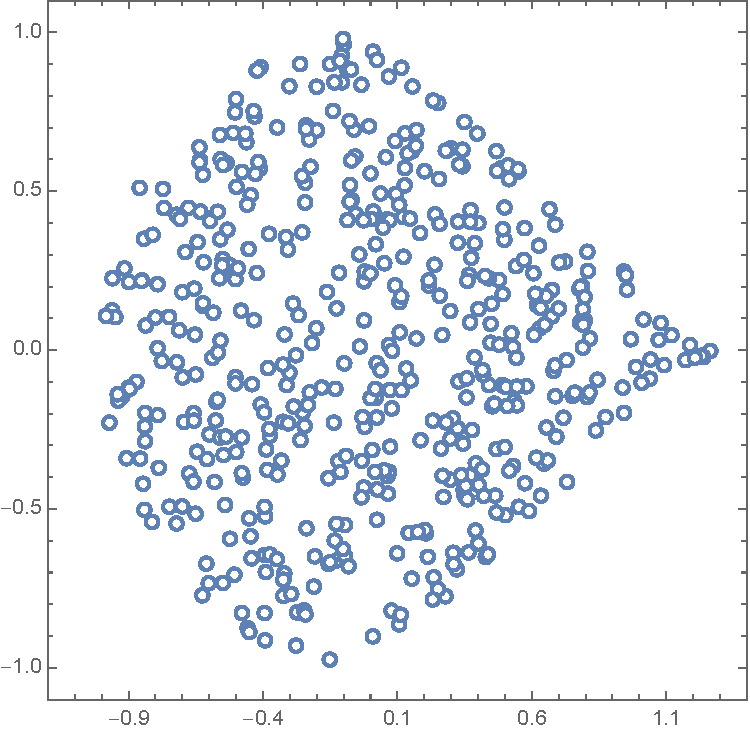
\includegraphics[width=\textwidth]{asym.pdf}
         \caption{}
         \label{fig:asym}
     \end{subfigure}
     \hfill
     \begin{subfigure}[b]{0.3\textwidth}
         \centering
         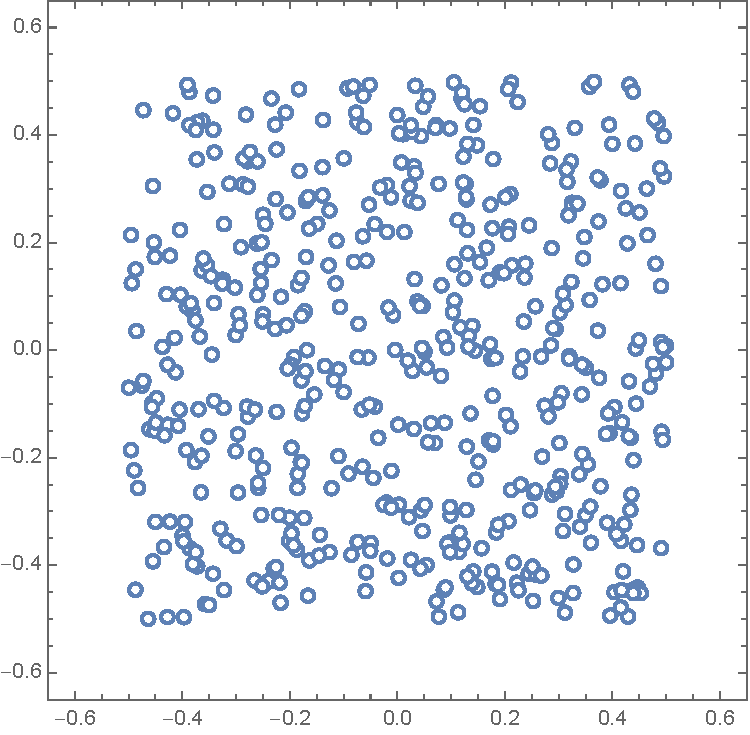
\includegraphics[width=\textwidth]{sqr.pdf}
         \caption{}
         \label{fig:sqr}
     \end{subfigure}
     \hfill
     \begin{subfigure}[b]{0.3\textwidth}
         \centering
         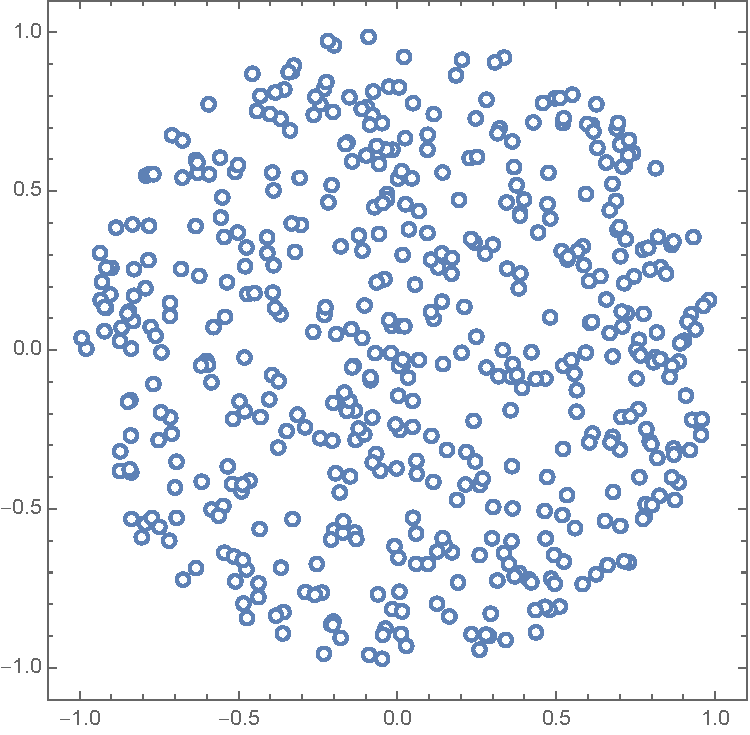
\includegraphics[width=\textwidth]{crc.pdf}
         \caption{}
         \label{fig:crc}
     \end{subfigure}
        \caption{Muestras de tamaño $500$ de (a) distribución asimétrica, (b) distribución uniforme sobre $[-0.5,0.5]^2$, (c) distribución uniforme sobre el disco unitario.}
        \label{fig:dists}
\end{figure}

\item A continuación se crearon $100$ muestras de tamaño $200$ de cada distribución llamando $X = \operatorname{Table}[\operatorname{Dist}[100],100]$ donde $\operatorname{Dist}$ se cambió según fuese el caso por $\operatorname{Asym}$, $\operatorname{Sqr}$, o $\operatorname{Crc}$, y sobre ellas se calcularon $100$ $p$-valores para la distribución para el test de permutación de simetría de signos, cada uno con $M = 1000$, llamando $p = \operatorname{Parallelize}[\operatorname{Table}[\operatorname{bp}[X[[i]],1000],{i,100}]]$.

\begin{enumerate}[label=(\roman*)]

\item De los $100$ $p$-valores calculados para la distribución asimétrica hubo $53$ $\geq 0.05$ y $35$ $\geq 0.1$. Aunque para esta distribución la hipótesis nula es falsa, la potencia del test parecería no ser suficiente dada una muestra de este tamaño.

\item De los $100$ $p$-valores calculados para la distribución uniforme sobre $[-0.5,0.5]^2$ hubo $93$ $\geq 0.05$ y $87$ $\geq 0.1$. Efectivamente para esta distribución donde la hipótesis nula es cierta el test es capaz de detectarlo.

\item De los $100$ $p$-valores calculados para la distribución uniforme sobre el disco unitario hubo $100$ $\geq 0.05$ y $97$ $\geq 0.1$. Efectivamente para esta distribución donde la hipótesis nula es cierta el test es capaz de detectarlo.

\end{enumerate}

\item Se repitió en este punto el paso anterior pero ahora con muestras de tamaño $500$ de cada distribución llamando $X = \operatorname{Table}[\operatorname{Dist}[250],100]$ donde $\operatorname{Dist}$ se cambió según fuese el caso por $\operatorname{Asym}$, $\operatorname{Sqr}$, o $\operatorname{Crc}$, y sobre ellas se calcularon $100$ $p$-valores para la distribución para el test de permutación de simetría de signos, cada uno con $M = 1000$, llamando $p = \operatorname{Parallelize}[\operatorname{Table}[\operatorname{bp}[X[[i]],1000],{i,100}]]$.

\begin{enumerate}[label=(\roman*)]

\item De los $100$ $p$-valores calculados para la distribución asimétrica hubo $3$ $\geq 0.05$ y $1$ $\geq 0.1$. Para este tamaño de muestra sí vemos la potencia del test, siendo éste capaz de detectar la falta de simetría de signos en esta distribución.

\item De los $100$ $p$-valores calculados para la distribución uniforme sobre $[-0.5,0.5]^2$ hubo $98$ $\geq 0.05$ y $95$ $\geq 0.1$. Efectivamente para esta distribución donde la hipótesis nula es cierta el test es capaz de detectarlo, y los resultados son aún mejores para este tamaño de muestra.

\item De los $100$ $p$-valores calculados para la distribución uniforme sobre el disco unitario hubo $99$ $\geq 0.05$ y $96$ $\geq 0.1$. Efectivamente para esta distribución donde la hipótesis nula es cierta el test es capaz de detectarlo, aunque curiosamente los resultados fueron ligeramente mejores para la muestra más pequeña.

\end{enumerate}

\item Luego se crearon $100$ muestras de tamaño $200$ de cada distribución llamando $X = \operatorname{Table}[\operatorname{Dist}[100],100]$ donde $\operatorname{Dist}$ se cambió según fuese el caso por $\operatorname{Asym}$, $\operatorname{Sqr}$, o $\operatorname{Crc}$, y sobre ellas se calcularon $100$ $p$-valores para la distribución para el test de permutación de simetría esférica, cada uno con $K = 5$ y $M = 1000$, llamando $p = \operatorname{Parallelize}[\operatorname{Table}[\operatorname{S2p}[X[[i]],5,1000],{i,100}]]$.

\begin{enumerate}[label=(\roman*)]

\item De los $100$ $p$-valores calculados para la distribución asimétrica hubo $73$ $\geq 0.05$ y $59$ $\geq 0.1$. Aunque para esta distribución la hipótesis nula es falsa, la potencia del test parecería no ser suficiente dada una muestra de este tamaño.

\item De los $100$ $p$-valores calculados para la distribución uniforme sobre $[-0.5,0.5]^2$ hubo $59$ $\geq 0.05$ y $48$ $\geq 0.1$. Aunque para esta distribución la hipótesis nula es falsa, la potencia del test parecería no ser suficiente dada una muestra de este tamaño.

\item De los $100$ $p$-valores calculados para la distribución uniforme sobre el disco unitario hubo $94$ $\geq 0.05$ y $90$ $\geq 0.1$. Efectivamente para esta distribución donde la hipótesis nula es cierta el test es capaz de detectarlo.

\end{enumerate}

\item Se repitió el paso anterior pero ahora con muestras de tamaño $500$ de cada distribución llamando $X = \operatorname{Table}[\operatorname{Dist}[250],100]$ donde $\operatorname{Dist}$ se cambió según fuese el caso por $\operatorname{Asym}$, $\operatorname{Sqr}$, o $\operatorname{Crc}$, y sobre ellas se calcularon $100$ $p$-valores para la distribución para el test de permutación de simetría de signos, cada uno con $K = 5$ y $M = 1000$, llamando $p = \operatorname{Parallelize}[\operatorname{Table}[\operatorname{S2p}[X[[i]],5,1000],{i,100}]]$.

\begin{enumerate}[label=(\roman*)]

\item De los $100$ $p$-valores calculados para la distribución asimétrica hubo $33$ $\geq 0.05$ y $23$ $\geq 0.1$. Para este tamaño de muestra  vemos un poco más la potencia del test, siendo éste capaz de detectar la falta de simetría esférica, sin embargo para esta distribución y este tamaño de muestra no es aún un gran resultado.

\item De los $100$ $p$-valores calculados para la distribución uniforme sobre $[-0.5,0.5]^2$ hubo $14$ $\geq 0.05$ y $7$ $\geq 0.1$. Para este tamaño de muestra  vemos ya la potencia del test, siendo éste capaz de detectar la falta de simetría esférica, y para esta distribución se logran mucho mejores resultados que para la anterior.

\item De los $100$ $p$-valores calculados para la distribución uniforme sobre el disco unitario hubo $95$ $\geq 0.05$ y $93$ $\geq 0.1$. Efectivamente para esta distribución donde la hipótesis nula es cierta el test es capaz de detectarlo, y en este caso sí se tiene que los resultados fueron ligeramente mejores para la muestra más grande.

\end{enumerate}

\item Concluimos que ambos tests de permutación tienen un muy buen comportamiento para distribuciones tales que la hipótesis nula es cierta, sin embargo su potencia cuando no lo es se ve afectada por el tamaño de la muestra. Para el test de simetría de signos parecería ser suficiente con tamaño $500$, mientras que para el test de simetría esférica dependerá también de la distribución, siendo un tamaño de $500$ suficiente para algo lo suficientemente asimétrico como el cuadrado, pero no para algo que pueda en alguna medida asemejar al disco unitario (como la mitad izquierda de la distribución asimétrica), para este último caso fue suficiente con un tamaño de muestra de $700$, con el cual se obtuvieron de $100$ $p$-valores $17$ $\geq 0.05$ y $7$ $\geq 0.1$.

\end{enumerate}

Como ya se mencionó, el hecho de que estos tests de permutaciones arrojen tan buenos resultados cuando $H_0$ es cierta y cuando $H_0$ es falsa y el tamaño de muestra es considerable nos da entonces que este es un método sensato y razonable para evaluar las hipótesis de simetría aquí consideradas, siempre y cuando se considere una muestra suficientemente grande.

Más allá de lo aquí realizado, esto también nos indica que los tests de permutación son una potente herramienta en la estadística no-paramétrica. Tomando un estadístico apropiado para una hipótesis, y hallando las permutaciones apropiadas para el mismo, es posible construir un test robusto y no paramétrico, y además de muy fácil implementación, al menos en cuanto a la escritura del código, pues debe mencionarse en este punto que los tests aquí realizados fueron computacionalmente muy costosos (por eso se paralelizó) al requerir el cálculo de cientas de miles de instancias de cada estadístico.

\nocite{FangSymmetricDistributions}

\bibliographystyle{unsrt}
\bibliography{references.bib}

\end{document}